% Sprint 4 — planification ch. 2 : BI, Power BI, KPI / GIMSI
\PFEChapterOpening{BI \& KPI}

\section{Introduction}

Ce chapitre présente le quatrième et dernier sprint fonctionnel principal, \emph{BI \& KPI}, tel qu'indiqué dans le tableau~\ref{tab:ch02-planification-sprints}. Il vise la \textbf{lecture consolidée} de la performance CSR pour le corporate~: tableaux de bord web, \textbf{comparaisons planifié / réalisé}, \textbf{exports}, \textbf{graphiques dynamiques} et socle pour \textbf{Power BI} et les \textbf{KPI GIMSI}. Le module \texttt{dashboard\_analytics} (préfixe \texttt{/api/dashboard}) et le paquet \texttt{powerbi\_integration} (\texttt{/api/powerbi}) structurent cette couche côté backend.

\section{Objectif attendu}

Fournir aux décideurs une vision \textbf{synthétique et actionnable} de l'avancement multi-sites, tout en permettant l'export et la réutilisation des données dans des outils d'analyse (Power BI, tableaux de direction). Les user stories des blocs \emph{Dashboard \& Reporting} (5.x), \emph{Reporting \& Power BI} (6.x) et \emph{KPI \& pilotage GIMSI} (10.x) du product backlog définissent ce sprint.

\section{Sprint Backlog}

Le tableau~\ref{tab:sprint-backlog-4} résume les tâches retenues.

% --- Sprint backlog — BI & KPI (sprint 4) ---
\begingroup
\PFETableSetup
\PFETableRowColors
\PFETableLongMargins
\PFETableArrayStretch
\begin{longtable}{@{}p{0.6cm}p{4.0cm}p{1.0cm}p{7.8cm}p{1.4cm}@{}}
\caption{Sprint backlog — BI \& KPI}\label{tab:sprint-backlog-4}\\
\toprule
\tableHeaderStyle \tableHeaderCell{ID} & \tableHeaderCell{User story} & \tableHeaderCell{Tâche} & \tableHeaderCell{Tâche (détail)} & \tableHeaderCell{Priorité} \\
\midrule
\endfirsthead
\multicolumn{5}{c}{\tablename\ \thetable{} — \textit{(suite)}} \\
\toprule
\tableHeaderStyle \tableHeaderCell{ID} & \tableHeaderCell{User story} & \tableHeaderCell{Tâche} & \tableHeaderCell{Tâche (détail)} & \tableHeaderCell{Priorité} \\
\midrule
\endhead
\midrule
\multicolumn{5}{r}{\textit{Suite page suivante\ldots}} \\
\endfoot
\bottomrule
\endlastfoot
1 & En tant qu'utilisateur corporate, je veux un tableau de bord consolidé afin de piloter la performance CSR & 1.1 & Agrégations multi-sites (\texttt{/api/dashboard})~: synthèses, graphiques d'activités, chronologie & +++++ \\
1 & En tant qu'utilisateur corporate, je veux un tableau de bord consolidé afin de piloter la performance CSR & 1.2 & Filtres (site, année, catégorie) et indicateurs de performance par site & +++++ \\
2 & En tant qu'utilisateur corporate, je veux comparer le planifié et le réalisé afin de mesurer les écarts & 2.1 & Endpoints ou sections dédiées aux écarts budget / volumes / jalons & +++++ \\
2 & En tant qu'utilisateur corporate, je veux comparer le planifié et le réalisé afin de mesurer les écarts & 2.2 & Représentations graphiques cohérentes avec les données validées & ++++ \\
3 & En tant qu'utilisateur corporate, je veux exporter les données afin de les partager & 3.1 & Export tabulaire ou fichiers (CSV / Excel) à partir des vues filtrées & ++++ \\
4 & En tant qu'utilisateur corporate, je veux visualiser des graphiques dynamiques afin de faciliter l'analyse & 4.1 & Composants front de visualisation (graphiques, cartes, top activités) branchés sur l'API dashboard & +++++ \\
5 & En tant que système, je veux synchroniser les données vers Power BI afin d'alimenter les tableaux de bord externes & 5.1 & Socle d'API \texttt{/api/powerbi} et stratégie de snapshot / rafraîchissement & ++++ \\
5 & En tant que système, je veux synchroniser les données vers Power BI afin d'alimenter les tableaux de bord externes & 5.2 & Sécurisation des accès et documentation des jeux de données publiés & +++ \\
6 & En tant qu'utilisateur corporate, je veux suivre les KPI GIMSI afin d'assurer l'amélioration continue & 6.1 & Formalisation des indicateurs retenus et calculs alignés sur le modèle de données CSR & +++++ \\
6 & En tant qu'utilisateur corporate, je veux suivre les KPI GIMSI afin d'assurer l'amélioration continue & 6.2 & Vues récapitulatives ou exports pour revue de direction & ++++ \\
\end{longtable}
\endgroup


\section{Analyse détaillée des besoins}

\subsection{Diagramme de cas d'utilisation}

La figure~\ref{fig:doc-ch6-1} illustre les cas du sprint \emph{BI \& KPI}.

\IfFileExists{figures/chapitre-06/diagramme-cas-utilisation-bi-kpi.png}{%
\begin{figure}[H]
  \centering
  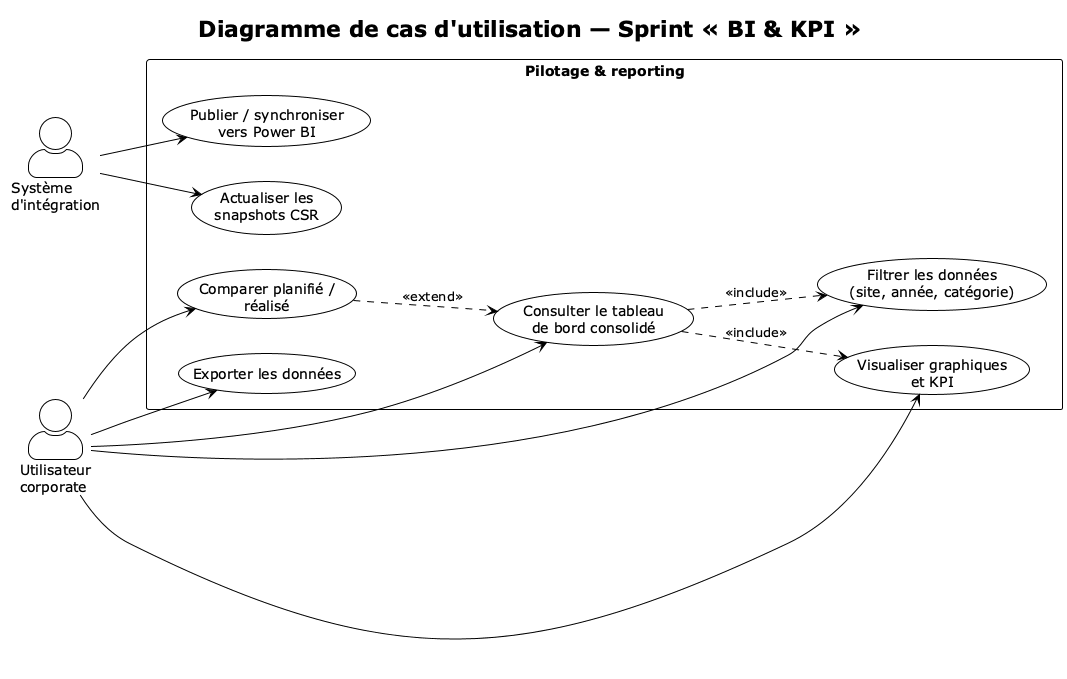
\includegraphics[width=0.92\linewidth]{figures/chapitre-06/diagramme-cas-utilisation-bi-kpi.png}
  \caption{Diagramme de cas d'utilisation — BI \& KPI.}
  \label{fig:doc-ch6-1}
\end{figure}%
}{%
\begin{figure}[H]
  \centering
  \fbox{\parbox{0.92\linewidth}{\centering\vspace{3.2cm}\textit{(Figure à insérer : \texttt{figures/chapitre-06/diagramme-cas-utilisation-bi-kpi.png})}\vspace{3.2cm}}}
  \caption{Diagramme de cas d'utilisation — BI \& KPI.}
  \label{fig:doc-ch6-1}
\end{figure}%
}

\subsection{Description textuelle du cas d'utilisation : «~Consulter le tableau de bord corporate~»}

Le tableau~\ref{tab:cu-tableau-de-bord} décrit le cas «~Consulter le tableau de bord corporate~».

\subsection{Description textuelle du cas d'utilisation : «~Exploiter les données pour le reporting et Power BI~»}

Le tableau~\ref{tab:cu-reporting-powerbi} décrit le cas «~Exploiter les données pour le reporting et Power BI~».

\begin{table}[htbp]
  \centering
  \small
  \caption{Description textuelle du cas d'utilisation : «~Consulter le tableau de bord corporate~»}
  \label{tab:cu-tableau-de-bord}
  \PFETableSetup
  \PFETableRowColors
  \PFETableArrayStretch
  \PFETableTabularXBegin
  \begin{tabularx}{\PFETableBlockWidth}{@{}>{\raggedright\arraybackslash}p{3.2cm} >{\raggedright\arraybackslash}X@{}}
    \tableHeaderStyle \tableHeaderCell{Champ} & \tableHeaderCell{Contenu} \\
    \textbf{Titre} & Consulter le tableau de bord corporate \\
    \textbf{Acteurs} & Utilisateur corporate (pilotage), éventuellement rôles restreints en lecture. \\
    \textbf{Objectif} &
      Offrir une vue consolidée des plans, activités et indicateurs clés pour suivre l'avancement CSR multi-sites et détecter les écarts. \\
    \textbf{Préconditions} &
      L'utilisateur est authentifié avec un périmètre corporate. Les données sources (plans validés, activités, réalisations) sont disponibles. \\
    \textbf{Postconditions} &
      Les indicateurs affichés reflètent les filtres choisis ; l'utilisateur peut basculer vers le détail d'un site ou exporter. \\
    \textbf{Scénario nominal} &
      L'utilisateur ouvre le tableau de bord, applique des filtres (année, site, catégorie), consulte les graphiques et tableaux, puis approfondit une zone sensible (top activités, chronologie, performance site). \\
    \textbf{Scénario alternatif} &
      \textbf{Données partielles :} affichage d'un bandeau d'avertissement si certains sites n'ont pas encore soumis de plan.\par\medskip
      \textbf{Timeout :} message invitant à réduire le périmètre temporel ou à réessayer. \\
  \end{tabularx}%
  \PFETableTabularXEnd
\end{table}

\begin{table}[htbp]
  \centering
  \small
  \caption{Description textuelle du cas d'utilisation : «~Exploiter les données pour le reporting et Power BI~»}
  \label{tab:cu-reporting-powerbi}
  \PFETableSetup
  \PFETableRowColors
  \PFETableArrayStretch
  \PFETableTabularXBegin
  \begin{tabularx}{\PFETableBlockWidth}{@{}>{\raggedright\arraybackslash}p{3.2cm} >{\raggedright\arraybackslash}X@{}}
    \tableHeaderStyle \tableHeaderCell{Champ} & \tableHeaderCell{Contenu} \\
    \textbf{Titre} & Exploiter les données pour le reporting et Power BI \\
    \textbf{Acteurs} & Système (synchronisation), utilisateur corporate (consommation des rapports). \\
    \textbf{Objectif} &
      Permettre l'alimentation de tableaux de bord Power BI et la réutilisation des agrégats CSR dans des analyses externes ou des revues périodiques. \\
    \textbf{Préconditions} &
      Jeux de données identifiés ; comptes ou clés d'accès Power BI conformes à la politique de sécurité de l'entreprise. \\
    \textbf{Postconditions} &
      Les rapports distants reflètent une photographie cohérente des données ; la fréquence de rafraîchissement est documentée. \\
    \textbf{Scénario nominal} &
      Le système exporte ou publie les agrégats vers le canal prévu ; l'utilisateur corporate ouvre le rapport Power BI et croise les vues avec d'autres sources internes si besoin. \\
    \textbf{Scénario alternatif} &
      \textbf{API Power BI en cours de complétion :} usage intermédiaire d'exports fichiers depuis le tableau de bord web.\par\medskip
      \textbf{Échec de synchronisation :} journal d'erreur et notification aux administrateurs. \\
  \end{tabularx}%
  \PFETableTabularXEnd
\end{table}


\section{Modélisation conceptuelle}

\subsection{Diagramme de classe}

La figure~\ref{fig:doc-ch6-2} schématise les agrégats et sources de données exposés au pilotage.

\IfFileExists{figures/chapitre-06/diagramme-classe-bi-kpi.png}{%
\begin{figure}[H]
  \centering
  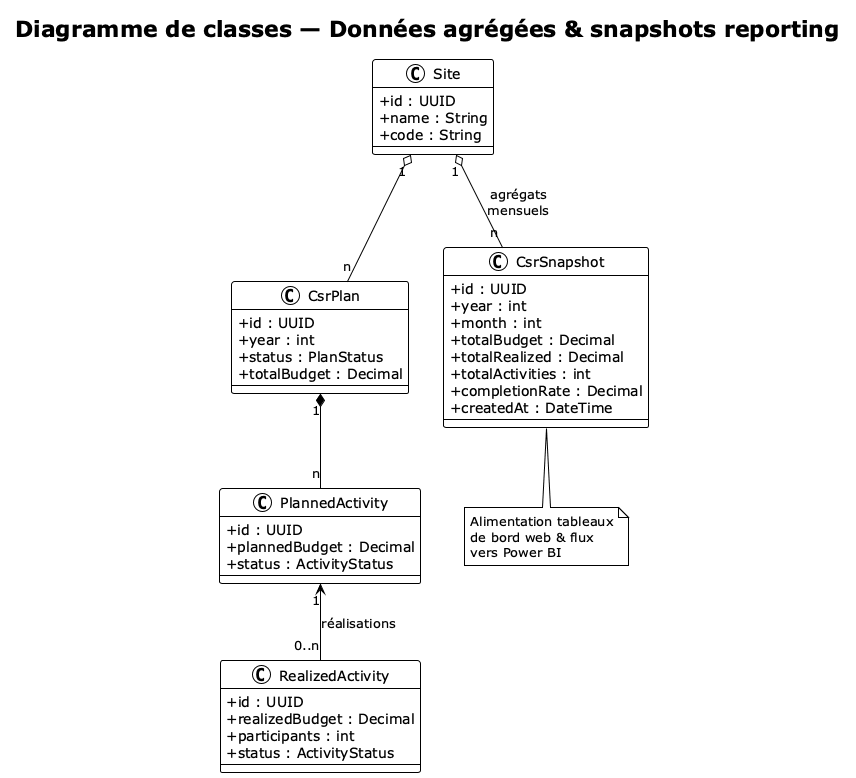
\includegraphics[width=0.92\linewidth]{figures/chapitre-06/diagramme-classe-bi-kpi.png}
  \caption{Diagramme de classe — BI \& KPI (agrégats, indicateurs).}
  \label{fig:doc-ch6-2}
\end{figure}%
}{%
\begin{figure}[H]
  \centering
  \fbox{\parbox{0.92\linewidth}{\centering\vspace{3.2cm}\textit{(Figure à insérer : \texttt{figures/chapitre-06/diagramme-classe-bi-kpi.png})}\vspace{3.2cm}}}
  \caption{Diagramme de classe — BI \& KPI (agrégats, indicateurs).}
  \label{fig:doc-ch6-2}
\end{figure}%
}

\subsection{Diagramme de séquence}

La figure~\ref{fig:doc-ch6-seq-dash} décrit le scénario «~Chargement du tableau de bord filtré~».

\IfFileExists{figures/chapitre-06/diagramme-sequence-dashboard-filtre.png}{%
\begin{figure}[H]
  \centering
  \includegraphics[width=0.92\linewidth]{figures/chapitre-06/diagramme-sequence-dashboard-filtre.png}
  \caption{Diagramme de séquence — chargement du tableau de bord.}
  \label{fig:doc-ch6-seq-dash}
\end{figure}%
}{%
\begin{figure}[H]
  \centering
  \fbox{\parbox{0.92\linewidth}{\centering\vspace{3.2cm}\textit{(Figure à insérer : \texttt{figures/chapitre-06/diagramme-sequence-dashboard-filtre.png})}\vspace{3.2cm}}}
  \caption{Diagramme de séquence — chargement du tableau de bord.}
  \label{fig:doc-ch6-seq-dash}
\end{figure}%
}

La figure~\ref{fig:doc-ch6-seq-export} illustre un export ou une extraction pour reporting.

\IfFileExists{figures/chapitre-06/diagramme-sequence-export-reporting.png}{%
\begin{figure}[H]
  \centering
  \includegraphics[width=0.92\linewidth]{figures/chapitre-06/diagramme-sequence-export-reporting.png}
  \caption{Diagramme de séquence — export / reporting.}
  \label{fig:doc-ch6-seq-export}
\end{figure}%
}{%
\begin{figure}[H]
  \centering
  \fbox{\parbox{0.92\linewidth}{\centering\vspace{3.2cm}\textit{(Figure à insérer : \texttt{figures/chapitre-06/diagramme-sequence-export-reporting.png})}\vspace{3.2cm}}}
  \caption{Diagramme de séquence — export / reporting.}
  \label{fig:doc-ch6-seq-export}
\end{figure}%
}

\section{Réalisation}

La figure~\ref{fig:doc-ch6-3} pourra présenter le tableau de bord corporate (cartes et graphiques).

\IfFileExists{figures/chapitre-06/ui-dashboard-corporate.png}{%
\begin{figure}[H]
  \centering
  \includegraphics[width=0.92\linewidth]{figures/chapitre-06/ui-dashboard-corporate.png}
  \caption{Interface : tableau de bord corporate.}
  \label{fig:doc-ch6-3}
\end{figure}%
}{%
\begin{figure}[H]
  \centering
  \fbox{\parbox{0.92\linewidth}{\centering\vspace{3.2cm}\textit{(Figure à insérer : \texttt{figures/chapitre-06/ui-dashboard-corporate.png})}\vspace{3.2cm}}}
  \caption{Interface : tableau de bord corporate.}
  \label{fig:doc-ch6-3}
\end{figure}%
}

La figure~\ref{fig:doc-ch6-4} pourra montrer une vue d'écarts ou de KPI / graphiques avancés.

\IfFileExists{figures/chapitre-06/ui-ecarts-kpi.png}{%
\begin{figure}[H]
  \centering
  \includegraphics[width=0.92\linewidth]{figures/chapitre-06/ui-ecarts-kpi.png}
  \caption{Interface : écarts planifié / réalisé ou KPI.}
  \label{fig:doc-ch6-4}
\end{figure}%
}{%
\begin{figure}[H]
  \centering
  \fbox{\parbox{0.92\linewidth}{\centering\vspace{3.2cm}\textit{(Figure à insérer : \texttt{figures/chapitre-06/ui-ecarts-kpi.png})}\vspace{3.2cm}}}
  \caption{Interface : écarts planifié / réalisé ou KPI.}
  \label{fig:doc-ch6-4}
\end{figure}%
}

\section{Tests et validation}

\subsection{Test}

Les tableaux~\ref{tab:ch6-scenario-dashboard-filtres} et~\ref{tab:ch6-scenario-ecarts-export} décrivent les scénarios de test principaux.

\begin{table}[htbp]
  \centering
  \small
  \caption{Scénario «~Tableau de bord avec filtres multi-sites~»}
  \label{tab:ch6-scenario-dashboard-filtres}
  \PFETableSetup
  \PFETableRowColors
  \PFETableArrayStretch
  \PFETableTabularXBegin
  \begin{tabularx}{\PFETableBlockWidth}{@{}>{\raggedright\arraybackslash}p{3.4cm} >{\raggedright\arraybackslash}X@{}}
    \tableHeaderStyle \tableHeaderCell{Élément} & \tableHeaderCell{Détail} \\
    \textbf{Titre de la fiche} &
      Cas d'erreur : «~Les indicateurs ne correspondent pas aux filtres ou restent vides.~» \\
    \textbf{Fonctionnalité associée} & Tableau de bord corporate (\texttt{/api/dashboard}). \\
    \textbf{Prérequis} &
      Utilisateur corporate authentifié.\par
      Jeu de données de test couvrant au moins deux sites et deux années. \\
    \textbf{Scénario} &
      1. Ouvrir le tableau de bord.\par
      2. Appliquer un filtre d'année puis un filtre de site.\par
      3. Vérifier les cartes (totaux, graphiques, top activités).\par
      4. Réinitialiser les filtres et contrôler la cohérence des agrégats globaux. \\
    \textbf{Cas d'erreur potentiel} &
      Combinaison de filtres sans données.\par
      Dérive des totaux après navigation rapide (cache client).\par
      Accès refusé pour un rôle non corporate. \\
    \textbf{Résultat attendu} &
      États vides explicites ; valeurs identiques à celles obtenues via requêtes de contrôle en base.\par
      Code HTTP et message adaptés en cas d'erreur. \\
  \end{tabularx}%
  \PFETableTabularXEnd
\end{table}

\begin{table}[htbp]
  \centering
  \small
  \caption{Scénario «~Comparaison planifié / réalisé et export~»}
  \label{tab:ch6-scenario-ecarts-export}
  \PFETableSetup
  \PFETableRowColors
  \PFETableArrayStretch
  \PFETableTabularXBegin
  \begin{tabularx}{\PFETableBlockWidth}{@{}>{\raggedright\arraybackslash}p{3.4cm} >{\raggedright\arraybackslash}X@{}}
    \tableHeaderStyle \tableHeaderCell{Élément} & \tableHeaderCell{Détail} \\
    \textbf{Titre de la fiche} &
      Cas d'erreur : «~L'export ne reflète pas les filtres ou échoue pour volumétrie élevée.~» \\
    \textbf{Fonctionnalité associée} & Écarts planifié / réalisé et export (US\,5.3--5.4). \\
    \textbf{Prérequis} &
      Plans et réalisations validés sur le périmètre filtré.\par
      Droit d'export corporate. \\
    \textbf{Scénario} &
      1. Afficher la vue des écarts pour une année donnée.\par
      2. Contrôler un échantillon de lignes par rapport au détail activité.\par
      3. Lancer l'export avec les mêmes filtres.\par
      4. Ouvrir le fichier et vérifier les en-têtes et le nombre de lignes. \\
    \textbf{Cas d'erreur potentiel} &
      Timeout sur gros volume.\par
      Séparateur ou encodage incorrect selon la locale.\par
      Données partiellement validées mélangées. \\
    \textbf{Résultat attendu} &
      Export reproductible ; message d'échec explicite avec suggestion (réduire la période, le nombre de sites). \\
  \end{tabularx}%
  \PFETableTabularXEnd
\end{table}


Les endpoints \texttt{/api/dashboard} et, selon l'avancement, \texttt{/api/powerbi} ont été testés avec \emph{Postman} et par contrôle croisé avec des requêtes d'agrégation sur un jeu de données de démonstration. Les figures~\ref{fig:ch6-postman-dashboard},~\ref{fig:ch6-postman-dashboard-site} et~\ref{fig:ch6-postman-powerbi} accueillent les captures.

\IfFileExists{figures/chapitre-06/postman-dashboard.png}{%
\begin{figure}[H]
  \centering
  \includegraphics[width=0.92\linewidth]{figures/chapitre-06/postman-dashboard.png}
  \caption{Tests Postman — agrégat dashboard (\texttt{/api/dashboard}).}
  \label{fig:ch6-postman-dashboard}
\end{figure}%
}{%
\begin{figure}[H]
  \centering
  \fbox{\parbox{0.92\linewidth}{\centering\vspace{3.2cm}\textit{(Figure à insérer : \texttt{figures/chapitre-06/postman-dashboard.png})}\vspace{3.2cm}}}
  \caption{Tests Postman — agrégat dashboard (\texttt{/api/dashboard}).}
  \label{fig:ch6-postman-dashboard}
\end{figure}%
}

\IfFileExists{figures/chapitre-06/postman-dashboard-filtre-site.png}{%
\begin{figure}[H]
  \centering
  \includegraphics[width=0.92\linewidth]{figures/chapitre-06/postman-dashboard-filtre-site.png}
  \caption{Tests Postman — dashboard avec filtre site / année.}
  \label{fig:ch6-postman-dashboard-site}
\end{figure}%
}{%
\begin{figure}[H]
  \centering
  \fbox{\parbox{0.92\linewidth}{\centering\vspace{3.2cm}\textit{(Figure à insérer : \texttt{figures/chapitre-06/postman-dashboard-filtre-site.png})}\vspace{3.2cm}}}
  \caption{Tests Postman — dashboard avec filtre site / année.}
  \label{fig:ch6-postman-dashboard-site}
\end{figure}%
}

\IfFileExists{figures/chapitre-06/postman-powerbi.png}{%
\begin{figure}[H]
  \centering
  \includegraphics[width=0.92\linewidth]{figures/chapitre-06/postman-powerbi.png}
  \caption{Tests Postman — couche Power BI (\texttt{/api/powerbi}).}
  \label{fig:ch6-postman-powerbi}
\end{figure}%
}{%
\begin{figure}[H]
  \centering
  \fbox{\parbox{0.92\linewidth}{\centering\vspace{3.2cm}\textit{(Figure à insérer : \texttt{figures/chapitre-06/postman-powerbi.png})}\vspace{3.2cm}}}
  \caption{Tests Postman — couche Power BI (\texttt{/api/powerbi}).}
  \label{fig:ch6-postman-powerbi}
\end{figure}%
}

\subsection{Validation}

La démonstration de fin de sprint a été réalisée avec le \emph{Product Owner} sur un périmètre multi-sites de démonstration. Les écarts résiduels entre indicateurs écran et exports ont été corrigés ; la feuille de route des compléments Power BI a été notée pour les évolutions post-livraison.

\section{Conclusion}

Ce sprint clôt la chaîne de livraison fonctionnelle prévue en quatre itérations en offrant aux métiers corporate les instruments de pilotage et de diffusion des résultats CSR.

La conclusion générale du mémoire, qui suit dans le document, synthétise les apports du projet et les perspectives.
